\documentclass{article}
\usepackage{realtristan}
\usepackage{setspace}
\title{General Relativity vs Light}
\author{Tristan Simpson}
\doublespacing
\begin{document}
\maketitle
\tableofcontents
\section{General Relativity}\label{sec:generalrelativity}
Albert Einstein's theory of general relativity is based on the idea that massive objects cause a distortion in space-time. The image below exhibits a clear representation of what that distortion looks like.\\\\
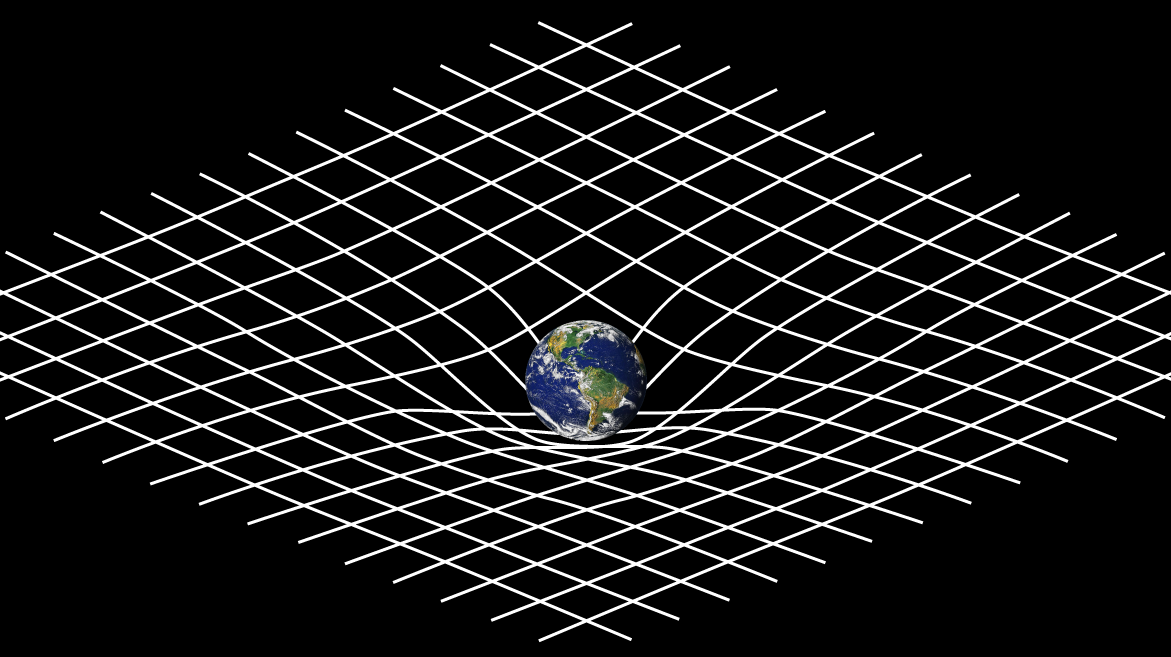
\includegraphics[scale=0.30]{images/general_relativity.png}


\section{Waves}
\subsection{Mechanical Waves}
A mechanical wave is an \hyperref[sec:oscillation]{oscillation} of matter and is responsible for the transfer of energy through a medium. (Note: Light is not a mechanical wave because it is not matter. The particles that make up light (\hyperref[sec:photons]{photons}) have no mass.)
\subsubsection{Different Types of Mechanical Waves}
In total there are \textbf{\textit{three}} general forms of mechanical waves. These waves are: Transverse Waves, Longitudinal Waves, and Combined Waves.
\subsection{Electromagnetic Waves}
Electromagnetic waves are those created by \hyperref[sec:oscillation]{oscillating} electric and magnetic fields. A great example of an electromagnetic wave is light. Light has two components: vertical and horizontal (electric and magentic field oscillation). This combination results in an electromagnetic wave.

\subsubsection{Different Types of Electromagnetic Waves}
In total there are \textbf{\textit{seven}} general forms of electromagnetic waves. These waves are: Radio Waves, Microwaves, Infrared, Visible, Ultraviolet, X-Ray, and Gamma Rays.
\subsection{Gravitational Waves}
First proposed by Albert Einstein in 1916 following his famously recognized \hyperref[sec:generalrelativity]{Theory of General Relativity}, gravitational waves are ripples in space-time (the fabled “fabric” of the Universe) caused by massive objects moving with extreme accelerations.\\\\
Over 20 years later in 1936, Albert Einstein and Nathan Rosen submitted a manuscript famously contradicting their theory of gravitational waves. This is because gravitational waves were theoretically possible, though they were thought to be physically impossible. \\\\
Gravitational waves were later proved to be existent, though it was determined that they're effect by the time they reached us would be so weak, detecting them would be nearly impossible. However, in 2015, the Laser Interferometer Gravitational-Wave Observatory (LIGO) detected gravitational waves from the collision of two black holes.\\\\
Gravitational waves are formed by, as an example, also described above, two black holes orbiting eachother, both getting closer and closer together until they collide.

\subsubsection{Gravitational Wave Visualization}
Gravitational waves are a very difficult concept to visualize. The following image is a basic visualization of gravitational waves. The two light-blue spheres are, for example, black holes. Their circulation around eachother leave ripples in spacetime.\\\\
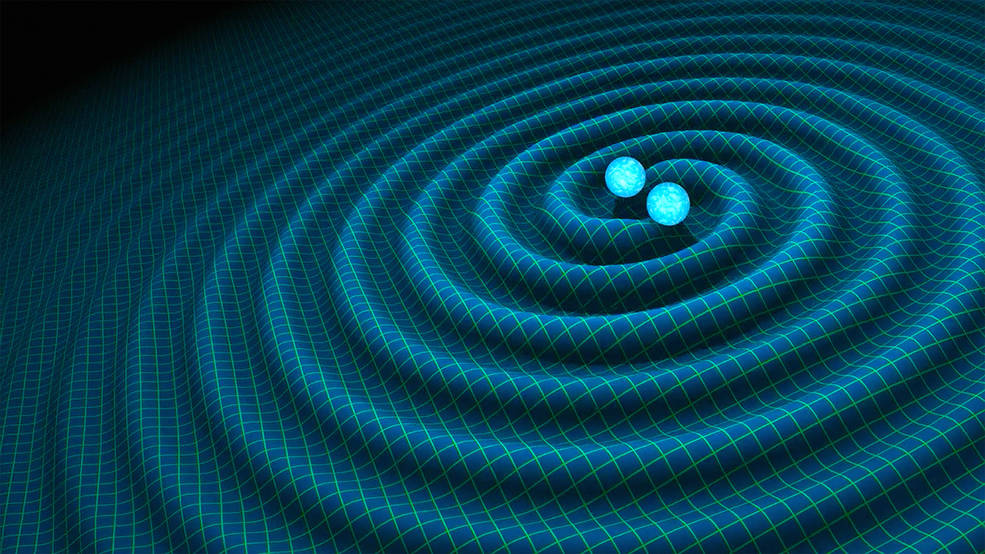
\includegraphics[scale=0.33]{images/gravitational_waves.png}

\subsection{Matter Waves}
Matter waves are a central part of the theory of quantum mechanics, being an example of wave-particle duality. All matter exhibits wave-like behavior. The matter waves describes the relationship between momentum and wavelength.


\section{Light}
\subsection{Wave Velocity}
The speed of an electromagnetic wave (therefore light waves) is dependant on its wave length and frequency. The measure of the waves velocity can be calculated by the following equation: $v = \lambda f$ where $v$ is the wave velocity, $\lambda$ is the wave length, and $f$ is the wave frequency. The units of velocity are meters per second (m/s).

\subsection{Components}
A light wave is made up of two components: electric and magnetic fields. These components can also be represented as vertical and horizontal vectors. These vectors later appear in the polarization of light waves.

\subsection{Polarization}
The polarization of a light wave allows for either the vertical or horizontal components of a wave to be eliminated. This elimination removes a minimum of $50\%$ of the lights' brightness.\\\\
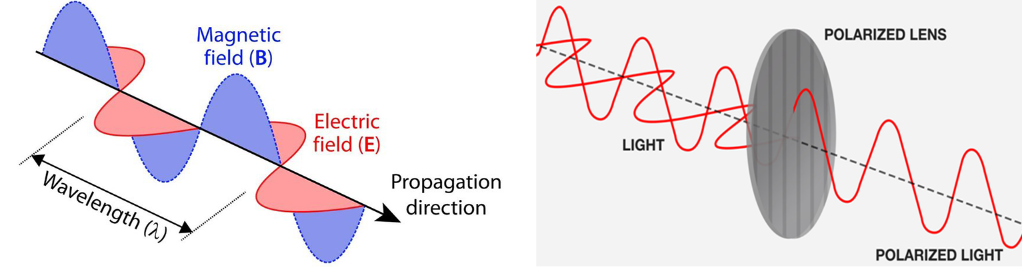
\includegraphics[scale=0.45]{images/polarization.png}
\subsection{Gravitational Lensing}\label{sec:gravitational_lensing}
Following Einstein's \hyperref[sec:generalrelativity]{Theory of General Relativity}, light can be bent by gravity. This bending is known as gravitational lensing. Because of gravitational lensing, the lights path around the electromagnetic field of an extremely large mass (eg. a neutron star) is curved.

\subsubsection{Gravitational Lensing Visualization}
The image below is a visualization of gravitational lensing. The light is being bent around the gravitational field of the black hole which reveals the cluster of stars behind it.\\\\
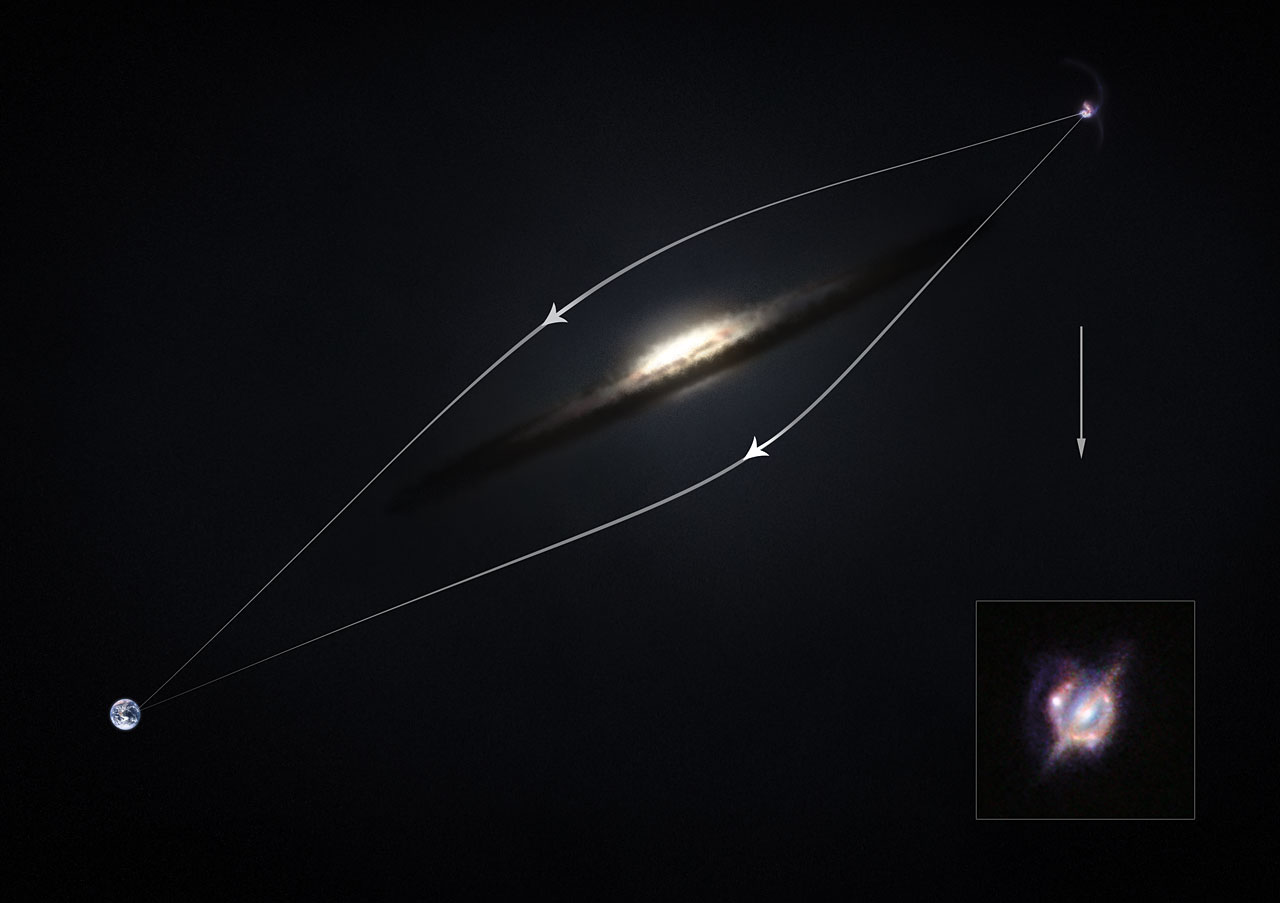
\includegraphics[scale=0.2]{images/grav_lensing.png}

\subsubsection{Gravitational Micro-Lensing}
Gravitational micro-lensing allows astronomers to detect objects that would otherwise be hidden in our vast universe (i.e. a black hole). A gravitational lens can occur when a huge amount of matter, like a cluster of galaxies, creates a gravitational field that distorts and magnifies the light from distant galaxies that are behind it but in the same line of sight. In 2019, the light of a star was observed to be distorted by the gravitational lensing of a black hole.

\subsubsection{So how does it work?}
The best way to describe gravitational lensing is through the visualization of a bowling ball moving around a circular pit. The bowling ball doesn't just simply fall into the pit because of its momentum and the curvature of the pit, instead, it curves around it. (i.e. light around an object of extremely large mass and distortion in space-time) See \hyperref[sec:generalrelativity]{Theory of General Relativity}

\subsection{Light - A Particle and Wave}
Not only is light a wave, but it is also a particle. This is known as wave-particle duality which is an essential theory derived from electromagnetics in quantum mechanics.

\subsubsection{Light as a Wave}
Combatting Isaac Newton's belief that light is a particle was Christiaan Huygens who had instead proposed that light was a wave. At the time Huygens wasn't able to prove his theory. It wasn't until 123 years later (1678 to 1801) when Thomas Young proved light was a wave through his Double Slit experiment.

\subsubsection{Light as a Particle}
Albert Einstein's quantum theory of light proposes that light is a series of \hyperref[sec:photons]{photons}, and the flow of \hyperref[sec:photons]{photons} is a wave. Einstein's essential point is that light's energy is directly related to its \hyperref[sec:oscillation]{oscillation} frequency. $E = \hbar\,\omega$ where $E$ is the energy of the \hyperref[sec:photons]{photon}, $\hbar$ is Planck's constant divided by $2\pi$ (i.e. $\frac{h}{2\pi}$), and $\omega$ is the angular frequency of the wave.\\\\


\section{Neutron Stars}

\subsection{Pulsars}



\section{Black Holes}
\subsection{Black Hole or Singularity?}
A common misconception is that the black hole is the same as the singularity. This is not the case. The singularity is the point of infinite density and curvature in spacetime. The black hole is the region of spacetime that is so warped by the singularity that nothing can escape it. The image below describes this relationship.\\\\
\begin{minipage}{0.5\textwidth}
    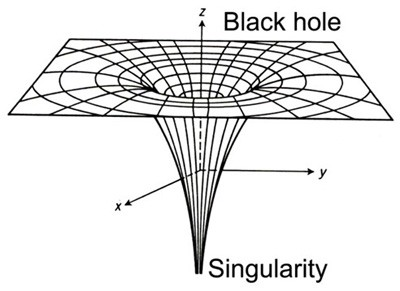
\includegraphics[scale=0.5]{images/black_hole.png}
\end{minipage}

\subsection{Light vs Black Holes}
It's impossible for anything to escape the event horizon of a black hole. This includes light. Light cannot escape because spacetime is so warped from the sheer mass of the black hole that it's relative region (See \hyperref[sec:generalrelativity]{Theory of General Relativity}) is so infinitely curved that it literally caves in on itself. This means that any direction the light tries to go to, it all just points back to the center of the black hole.
However, because of the black holes distortion in spacetime, light bends around it's relative dip. See \hyperref[sec:gravitational_lensing]{Gravitational Lensing}

\subsection{Solar Mass Measurement}
The mass of a black hole is measured by it's factor of solar mass. A solar mass is the mass of our sun which is \hyperref[constants]{$\approx 1.989 \times 10^{30}$} kilograms. Therefore, a black hole with the mass of two solar masses would be $\approx 2(1.989 \times 10^{30}) \approx 3.978 \times 10^{30}$ kilograms.

\subsection{Schwarzschild Radius}
\subsubsection{What is it?}
The Schwarzschild radius is the radius of the event horizon surrounding a black hole. Any large mass that gets compressed smaller than its Schwarzschild radius turns into a black hole. Only a black hole requires an objects velocity to be greater than the speed of light to escape it's gravitational pull.

\subsubsection{Visualization}
The following image is a visualization of a black hole and it's Schwarzschild radius. The singularity is the actual black hole. The event horizon is from the blue dotted circle to the singularity in the middle. Schwarzschild radius describes the distance from the outer of the singularity to the edge of the event horizon.\\\\
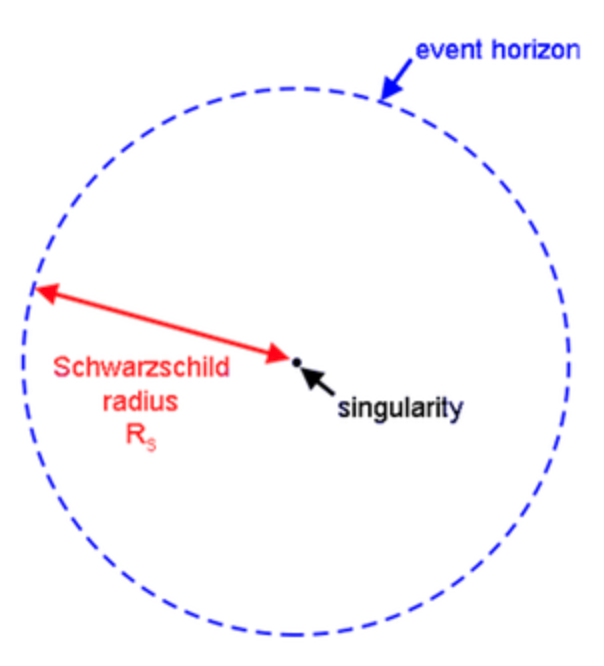
\includegraphics[scale=0.4]{images/schwarzschild_radius.png}

\subsubsection{Schwarzschild Radius Equation}\label{sec:schwarzschild_radius_equation}
The Schwarzschild radius is calculated using the equation: $R_{S} = \frac{2GM}{c^2}$ where $R_{S}$ is the Schwarzschild radius, $G$ is the gravitational constant (\hyperref[sec:constants]{$6.67 \times 10^{-11}\;\frac{Nm^2}{kg^2}$}), $M$ is the mass of the object, and $c$ is the speed of light (\hyperref[sec:constants]{$\approx 299, 792, 458\;\frac{m}{s}$}). The units of the Schwarzschild radius are meters (m).

\subsection{Gravitational Force}
The gravitational force of a black hole can be calculated using the equation: $F_g = \left(\frac{G\times m_1m_2}{r^2}\right)$ where $F_g$ is the gravitational force, $G$ is Newtons gravitational constant (\hyperref[sec:constants]{$6.67 \times 10^{-11}\;\frac{Nm^2}{kg^2}$}), $m_1$ is the mass of the black hole, $m_2$ is the mass of the object being pulled in, and $r$ is the radius of the black hole (found using the \hyperref[sec:schwarzschild_radius_equation]{Schwarzschild Radius Equation}). The units for gravitational force in this solution are Newtons per Kilogram ($\frac{N}{kg}$).

\subsection{Solving for the Gravitational Force}
\subsubsection{Variables}
\begin{itemize}
    \item $Given:\; G = 6.67 \times 10^{-11}\;\frac{Nm^2}{kg^2}$
    \item $Given:\; m_1 = 1.989\times 10^{30}\;kg$
    \item $Given:\; m_2 = 1\;kg$
    \item $Solved\; for: R_S = 2.95 \times 10^{3}\;m$
    \item $Find: F_g = \left(\frac{Gm_1m_2}{r^2}\right)$
\end{itemize}\leavevmode

\subsubsection{Solve for Schwarzschild Radius}
\begin{align*}
     & \therefore\;\; R_{S} = \left(\frac{2GM}{c^2}\right) = \left(\frac{2(6.67 \times 10^{-11})(1.989\times 10^{30})}{(299,792,458)^2}\right) \approx 2.95 \times 10^{3} \;m \\\\
     & \therefore\;\; The\; Schwarzschild\; Radius\; (R_{S})\; is\; approximately\; 2.95 \times 10^{3} \;m
\end{align*}\leavevmode

\subsubsection{Solve for Gravitational Force}
After solving for the Schwarzschild radius, we can subtitute it into Isaac Newtons law of universal gravitational equation which will in return give us the gravitational force.
\begin{align*}
     & \therefore\;\; F_g = \left(\frac{Gm_1m_2}{r^2}\right) = \left(\frac{(6.67 \times 10^{-11})(1.989\times 10^{30})(1)}{{(2.95 \times 10^{3})}^2}\right) \approx 4.5 \times 10^{13} \;\frac{N}{kg} \\\\
     & \therefore\;\; The\; Gravitational\; Force\; (F_g)\; is\; approximately\; 4.5 \times 10^{13} \;\frac{N}{kg}
\end{align*}

\subsubsection{Black Hole Gravitational Force on Light}
Discovered by Karl Schwarzschild, the gravitational force on light of a spinning black hole can be calculated using the equation $F_g = \left(\frac{hc^3}{GM\lambda}\right)$ for a spinning black hole or $F_g = \left(\frac{hc^3}{4GM\lambda}\right)$ for a non-spinning black hole. The variable $F_g$ is the gravitational force, $h$ is Planck's constant (\hyperref[sec:constants]{$6.626 \times 10^{-34}\;\frac{m^2kg}{s}$}), $c$ is the speed of light (\hyperref[sec:constants]{$\approx 299, 792, 458\;\frac{m}{s}$}), $G$ is Newton's gravitational constant (\hyperref[sec:constants]{$6.67 \times 10^{-11}\;\frac{Nm^2}{kg^2}$}), $M$ is the mass of the black hole, and $\lambda$ is the wavelength of the light in meters ($\approx 5.52\times 10^{-7}\; m$)

\subsection{Gravity in a Black Hole vs Earth}
The gravitational force ($F_g$) in a black hole is approximately $4.5 \times 10^{13}\; \frac{N}{kg}$ whereas the gravitational force here on earth is approximately $9.81\; \frac{N}{kg}$. This means that the gravitational force in a black hole is approximately $4.6 \times 10^{12}\; \frac{N}{kg}$ times greater than the gravitational force here on earth.

\subsection{Black Hole Time Dilation}
\subsubsection{Mass of it's Singularity}
A singularity is a point in space where extremely large amounts of matter are crushed into an infinitely small volume and density. Using either it's density or volume we can calulate it's mass using the equation: $m = \rho v$ where $m$ is the mass, $\rho$ is the density, and $v$ is the volume. Since $\infty$ is not quantifyable, any substitution of it in any equation produces a result of $\pm \infty$ or 0. Therefore, we can assume that the mass of the singularity is $\infty$.

\subsubsection{Gravitational Time Dilation}
The equation for gravitational time dilation is $\Delta t\prime = \Delta t\times\sqrt{(1-\frac{2GM}{rc^2})}$ where $\Delta t\prime$ is the time dilation, $\Delta t$ is the time in reference (i.e. an hour), $G$ is the gravitational constant, $M$ is the mass of the object, $r$ is the distance from the object to the center of the object, and $c$ is the speed of light.\\\\
In order for this equation to be valid, the object must be in a vacuum of space, thus we must increment our Schwarzschild radius ($R_{S}$) by a small amount, otherwise our calculations will result in an imaginary number (i.e. $\sqrt{-1}$).

\subsubsection{Gravitational Time Dilation of a Singularity}
By the time you've reached the singularity in a black hole, you'd be trapped in time. This is because as you come closer to an object of extremely large mass, because of it's distortion in spacetime (See \hyperref[sec:generalrelativity]{Theory of General Relativty}), time moves slower. Therefore we can assume that because the mass of a singularity is infinite, time in a singularity does not increment. \\\\
Since we know that the mass of the singularity is infinite, we can substitute $\infty$ into the gravitational time dilation equation as $M$ and immediately solve the equation since our mass ($M = \infty$) is not quantifyable. Because of this, the time dilation of a singularity ($\Delta t\prime$) is infinite.

\subsubsection{Gravitational Time Dilation of a Black Hole}
To solve for the gravitational time dilation of a black hole we can use the same formula: $\Delta t\prime = \Delta t\times\sqrt{(1-\frac{2GM}{rc^2})}$ except we increase the Schwarzschild radius ($R_{S}$) by a small amount to accompany the requisite of being in a vacuum of space for our equation to be valid. In this case we're going to increase the radius from $2.95 \times 10^{3}\; m \to 3.00 \times 10^{3}\; m$.
\vspace{-0.2cm}
\begin{align*}
    \Delta t\prime & = \Delta t\times\sqrt{(1-\frac{2GM}{rc^2})}                                                                          \\
                   & = 1\; hour \times\sqrt{(1-\frac{2(6.67 \times 10^{-11})(1.989\times 10^{30})}{(3.00 \times 10^{3})(299,792,458)^2})} \\
                   & \approx \sqrt{1.592\times10^{-2}}                                                                                    \\
                   & \approx 1.26 \times 10^{-1} \; hours
\end{align*}
Therefore for every one hour on earth, $\approx 1.26 \times 10^{-1}$ hours pass on the outards of a black hole.
If we want to calculate the gravitational time dilation of a spacecraft orbiting the black hole, we just add the distance from the spacecraft to our Schwarzschild radius. $R_{SC + S} = R_S + R_{SC}$ where $R_{SC}$ is the spacecraft distance.

\subsubsection{Relative Velocity Time Dilation}
When something is moving faster than something else, time dilation is experienced due to the discrepancy between velocities. The equation for relative velocity time dilation is $\Delta t\prime = \left(\Delta t \div \sqrt{1 - (v^2 \div c^2)}\right)$ where $\Delta t\prime$ is the time dilation, $\Delta t$ is the time interval (i.e. an hour), $v$ is the velocity of the object, and $c$ is the speed of light.
We can assume that our variable \textbf{\textit{v}} is equal to \textbf{\textit{c}} since the velocity of an object inside a black hole is equal to the speed of light. This leaves us with:\\
\vspace{-0.2cm}
\begin{minipage}{0.5\textwidth}
    \begin{align*}
        \Delta t\prime & = \left(\Delta t \div \sqrt{1 - (c^2 \div c^2)}\right) \\
                       & = \left(1 \div \sqrt{1 - 1}\right)                     \\
                       & = \left(1 \div \sqrt{0}\right)                         \\
                       & = \left(1 \div 0\right)                                \\
                       & = undefined
    \end{align*}
\end{minipage}
\begin{minipage}{0.5\textwidth}
    Therefore, calculating the relative velocity time dilation in a black hole is impossible. Our result describes that on earth $undefined$ (assuming $\infty$) hours had passed for the object to travel for one hour inside the black hole.
\end{minipage}\leavevmode\\\\

\subsection{Quarks in Black Holes}


\subsection{Event Horizon}


\subsection{Hawking Radiation}
Hawking Radiation is what makes black holes eventually disappear. To accomodate for the law of conservation of energy, the black hole uses it's mass to spew out hawking radiation. Overtime as the hawking radiation builds up, the black hole will eventually disappear. (Could this be the birth of a white hole?). (Clear this section up and clarify and prove some stuff.)

\subsection{Black Hole Information Paradox}




\section{White Holes}




\section{Worm Holes}




\section{Constants}\label{sec:constants}
\begin{itemize}
    \item Speed of Light: $c \approx 299,792,458\;\frac{m}{s}$
    \item Gravitational Constant: $G \approx 6.67 \times 10^{-11}\;\frac{Nm^2}{kg^2}$
    \item Plancks Constant (Energy and Frequency): $\approx 6.626\times 10^{-34}\frac{m^2kg}{s}$
    \item One Solar Mass: $\approx 1.989 \times 10^{30}$ kg
\end{itemize}

\section{Word Bank}
\subsection{Oscillation}\label{sec:oscillation}
The movement back and forth at a regular speed. Regular variation in magnitude or position around a central point.

\subsection{Photons}\label{sec:photons}
A packet of electromagnetic energy with no mass nor any charge. A photon is a particle. A photon is the smallest unit of light.

\end{document}